\subsubsection*{U\+ML state machines (main source wikipedia)}

The Unified Modeling Language has a notation for describing state machines. U\+ML state machines overcome the limitations of traditional finite state machines while retaining their main benefits.

 
\begin{DoxyImage}
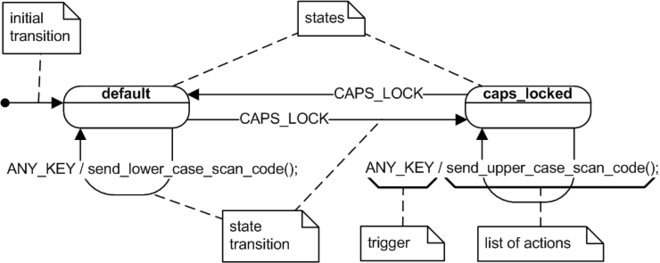
\includegraphics[width=10cm]{basic_uml_state_chart.png}
\caption{Basic U\+ML state chart}
\end{DoxyImage}


U\+ML state machines introduce the new concepts of hierarchically nested states and orthogonal regions, while extending the notion of actions. U\+ML state machines have the characteristics of both Mealy machines and Moore machines. They support actions that depend on both the state of the system and the triggering event, as in Mealy machines, as well as entry and exit actions, which are associated with states rather than transitions, as in Moore machines.

\subsubsection*{Supported features in this implementation (main source wikipedia)}

\paragraph*{Events}

An event is something that happens that affects the system. Strictly speaking, in the U\+ML specification, the term event refers to the type of occurrence rather than to any concrete instance of that occurrence.

An event can have associated parameters, allowing the event instance to convey not only the occurrence of some interesting incident but also quantitative information regarding that occurrence.

An event instance outlives the instantaneous occurrence that generated it and might convey this occurrence to one or more state machines. Once generated, the event instance goes through a processing life cycle that can consist of up to three stages. First, the event instance is received when it is accepted and waiting for processing (e.\+g., it is placed on the event queue). Later, the event instance is dispatched to the state machine, at which point it becomes the current event. Finally, it is consumed when the state machine finishes processing the event instance. A consumed event instance is no longer available for processing.

\paragraph*{States}

A state captures the relevant aspects of the system\textquotesingle{}s history very efficiently. To relate this concept to programming, this means that instead of recording the event history in a multitude of variables, flags, and convoluted logic, you rely mainly on just one state variable that can assume only a limited number of a priori determined values. The value of the state variable crisply defines the current state of the system at any given time. The concept of state reduces the problem of identifying the execution context in the code to testing just the state variable instead of many variables, thus eliminating a lot of conditional logic. Moreover, switching between different states

\paragraph*{Guard conditions}

Guard conditions (or simply guards) are Boolean expressions evaluated dynamically based on the value of extended state variables and event parameters. Guard conditions affect the behavior of a state machine by enabling actions or transitions only when they evaluate to T\+R\+UE and disabling them when they evaluate to F\+A\+L\+SE. In the U\+ML notation, guard conditions are shown in square brackets.

The need for guards is the immediate consequence of adding memory extended state variables to the state machine formalism. Used sparingly, extended state variables and guards make up a powerful mechanism that can simplify designs. But don not let the fancy name (\char`\"{}guard\char`\"{}) and the concise U\+ML notation fool you. When you actually code an extended state machine, the guards become the same I\+Fs and E\+L\+S\+Es that you wanted to eliminate by using the state machine in the first place. Too many of them, and you will find yourself back in square one (\char`\"{}spaghetti code\char`\"{}), where the guards effectively take over handling of all the relevant conditions in the system.

\paragraph*{Actions and transitions}

When an event instance is dispatched, the state machine responds by performing actions, such as changing a variable, performing I/O, invoking a function, generating another event instance, or changing to another state. Any parameter values associated with the current event are available to all actions directly caused by that event. Switching from one state to another is called state transition, and the event that causes it is called the triggering event, or simply the trigger.

\paragraph*{Entry and exit actions}

Every state in a U\+ML statechart can have optional entry actions, which are executed upon entry to a state, as well as optional exit actions, which are executed upon exit from a state. Entry and exit actions are associated with states, not transitions.

 
\begin{DoxyImage}
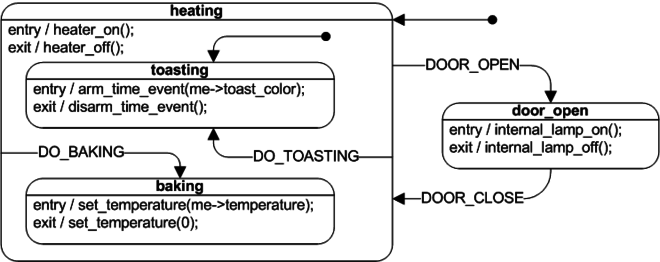
\includegraphics[width=10cm]{entry_exit_actions.png}
\caption{Entry/\+Exit Actions}
\end{DoxyImage}


Regardless of how a state is entered or exited, all its entry and exit actions will be executed. Because of this characteristic, statecharts behave like Moore machines. The U\+ML notation for state entry and exit actions is to place the reserved word \char`\"{}entry\char`\"{} (or \char`\"{}exit\char`\"{}) in the state right below the name compartment, followed by the forward slash and the list of arbitrary actions.

\paragraph*{Internal transitions}

Very commonly, an event causes only some internal actions to execute but does not lead to a change of state (state transition). In this case, all actions executed comprise the internal transition. In the absence of entry and exit actions, internal transitions would be identical to self-\/transitions (transitions in which the target state is the same as the source state).

 
\begin{DoxyImage}
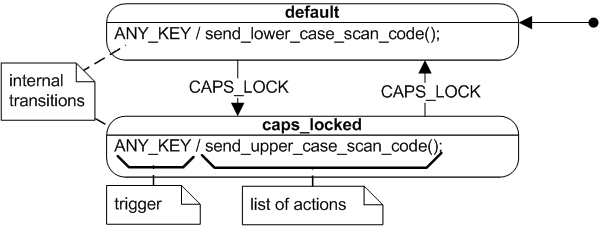
\includegraphics[width=10cm]{internal_transition.png}
\caption{Internal Transitions}
\end{DoxyImage}


In fact, in a classical Mealy machine, actions are associated exclusively with state transitions, so the only way to execute actions without changing state is through a self-\/transition. However, in the presence of entry and exit actions, as in U\+ML statecharts, a self-\/transition involves the execution of exit and entry actions and therefore it is distinctively different from an internal transition. 